\documentclass[border=12pt]{standalone}
\usepackage{tikz}
\usetikzlibrary{arrows.meta, positioning}
\begin{document}
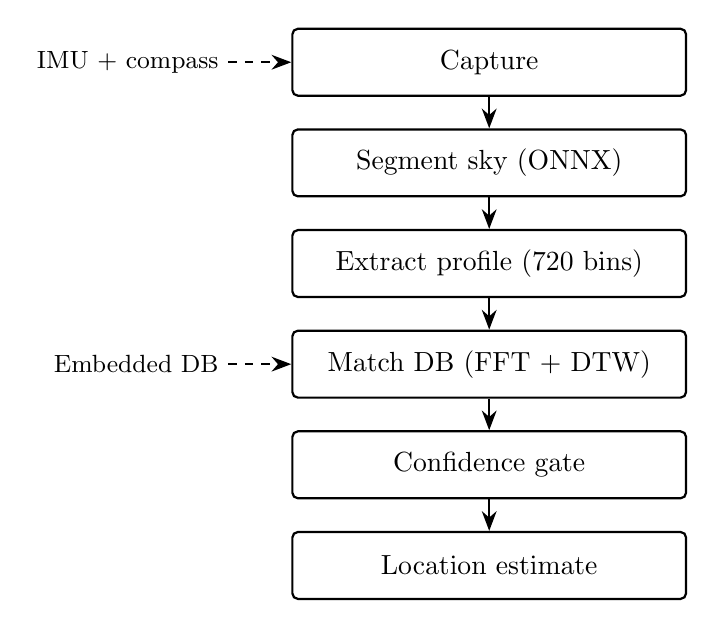
\begin{tikzpicture}[
    node distance=0.5cm,
    box/.style={rectangle, draw=black, thick, minimum width=5cm, minimum height=0.85cm,
                text centered, font=\normalsize, rounded corners=2pt},
    arr/.style={-{Stealth[length=2.5mm]}, thick},
]

\node[box] (cam) {Capture};
\node[box, below=0.4cm of cam] (seg) {Segment sky (ONNX)};
\node[box, below=0.4cm of seg] (prof) {Extract profile (720 bins)};
\node[box, below=0.4cm of prof] (match) {Match DB (FFT + DTW)};
\node[box, below=0.4cm of match] (gate) {Confidence gate};
\node[box, below=0.4cm of gate] (loc) {Location estimate};

\draw[arr] (cam) -- (seg);
\draw[arr] (seg) -- (prof);
\draw[arr] (prof) -- (match);
\draw[arr] (match) -- (gate);
\draw[arr] (gate) -- (loc);

% Side inputs
\node[left=0.8cm of cam, font=\small] (imu) {IMU + compass};
\draw[arr, dashed] (imu) -- (cam);

\node[left=0.8cm of match, font=\small] (db) {Embedded DB};
\draw[arr, dashed] (db) -- (match);

\end{tikzpicture}
\end{document}
